\let\negmedspace\undefined
\let\negthickspace\undefined
\documentclass[journal]{IEEEtran}
\usepackage[a5paper, margin=10mm, onecolumn]{geometry}
%\usepackage{lmodern} % Ensure lmodern is loaded for pdflatex
\usepackage{tfrupee} % Include tfrupee package

\setlength{\headheight}{1cm} % Set the height of the header box
\setlength{\headsep}{0mm}     % Set the distance between the header box and the top of the text

\usepackage{gvv-book}
\usepackage{comment}
\usepackage{gvv}
\usepackage{cite}
\usepackage{amsmath,amssymb,amsfonts,amsthm}
\usepackage{algorithmic}
\usepackage{graphicx}
\usepackage{textcomp}
\usepackage{xcolor}
%\usepackage{txfonts}
\usepackage{listings}
\usepackage{enumitem}
\usepackage{mathtools}
\usepackage{gensymb}
\usepackage{comment}
\usepackage[breaklinks=true]{hyperref}
\usepackage{tkz-euclide} 
\usepackage{listings}
% \usepackage{gvv}                                        
\def\inputGnumericTable{}                                 
\usepackage[latin1]{inputenc}                                
\usepackage{color}                                            
\usepackage{array}                                            
\usepackage{longtable}                                       
\usepackage{calc}                                             
\usepackage{multirow}                                         
\usepackage{hhline}                                           
\usepackage{ifthen}                                           
\usepackage{lscape}
\usepackage{circuitikz}
\tikzstyle{block} = [rectangle, draw, fill=blue!20, 
    text width=4em, text centered, rounded corners, minimum height=3em]
\tikzstyle{sum} = [draw, fill=blue!10, circle, minimum size=1cm, node distance=1.5cm]
\tikzstyle{input} = [coordinate]
\tikzstyle{output} = [coordinate]


\begin{document}

\bibliographystyle{IEEEtran}
\vspace{3cm}

\title{12.235}
\author{EE25BTECH11013 - Bhargav}
\maketitle
    {\let\newpage\relax\maketitle}

\renewcommand{\thefigure}{\theenumi}
\renewcommand{\thetable}{\theenumi}
\setlength{\intextsep}{10pt} % Space between text and floats

\numberwithin{equation}{enumi}
\numberwithin{figure}{enumi}
\renewcommand{\thetable}{\theenumi}

\textbf{Question}: \\
A system of equations represented as
\begin{align}
\myvec{1 & -1 & 2 \\ 2 & 1 & 4 \\ 1 & 3 & 1}\myvec{x_1 \\ x_2 \\ x_3} = \myvec{4 \\ y \\ 3} is,
\end{align}
\begin{enumerate}
\item consistent and has a unique solution
\item inconsistent and has no solution
\item consistent and infinite solution
\item inconsistent and has unique solution
\end{enumerate}
\solution \\
This can be represented as an augmented matrix and can be solved by using Gaussian elimination.
\begin{align}
\augvec{3}{1}{1 & -1 & 2 & 4\\ 2 & 1 & 4 & y\\ 1 & 3 & 1 & 3} \xleftrightarrow[R_3 \leftarrow R_3 - R_1]{R_2 \leftarrow R_2 - 2R_1}\augvec{3}{1}{1 & -1 & 2 & 4 \\ 0 & 3 & 0 & y-8 \\ 0 & 4 & -1 & -1}
\end{align}
\begin{align}
\xleftrightarrow[R_3 \leftarrow R_3 - 4R_2]{R_2 \leftarrow \frac{R_2}{3}} \augvec{3}{1}{1 & -1 & 2 & 4\\ 0 & 1 & 0 & \frac{y-8}{3} \\ 0 & 0 & -1 & \frac{29-4y}{3}} \xleftrightarrow[R_1 \leftarrow R_1 - 2R_3]{R_3 \leftarrow -R_3}
\end{align}
\begin{align}
\augvec{3}{1}{1 & -1 & 0 & \frac{70- 8y}{3} \\ 0 & 1 & 0 & \frac{y-8}{3}\\ 0 & 0 & 1 & \frac{4y-29}{3}} \xleftrightarrow{R_1 \leftarrow R_1 + R_2} \augvec{3}{1}{1 & 0 & 0 & \frac{62 - 7y}{3} \\ 0 & 1 & 0 & \frac{y-8}{3} \\ 0 & 0 & 1 & \frac{4y - 29}{3}}
\end{align}
\begin{align}
\myvec{x_1 \\ x_2 \\ x_3} = \myvec{\frac{62 - 7y}{3} \\ \frac{y-8}{3} \\ \frac{4y - 29}{3}}
\end{align}
Since $y  \in \mathbf{R}$, we can conclude that there exists a unique solution and the system of equations is consistent. \\

Option (1) is the correct answer \\ \\ 

This can be verified by finding the point of intersection of 3 planes:\\
As an example, take $y = 8$
\begin{align}
x_1 - x_2 + 2x_3 = 4
\end{align}
\begin{align}
2x_1 + x_2 + 4x_3 = 8
\end{align}
\begin{align}
x_1 + 3x_2 + x_3 = 3
\end{align}

The point of intersection of the planes from \brak{4.4} is
\begin{align}
\myvec{x_1 \\ x_2 \\ x_3} = \myvec{2 \\ 0 \\ 1}
\end{align}

\begin{figure}[H]
    \centering
    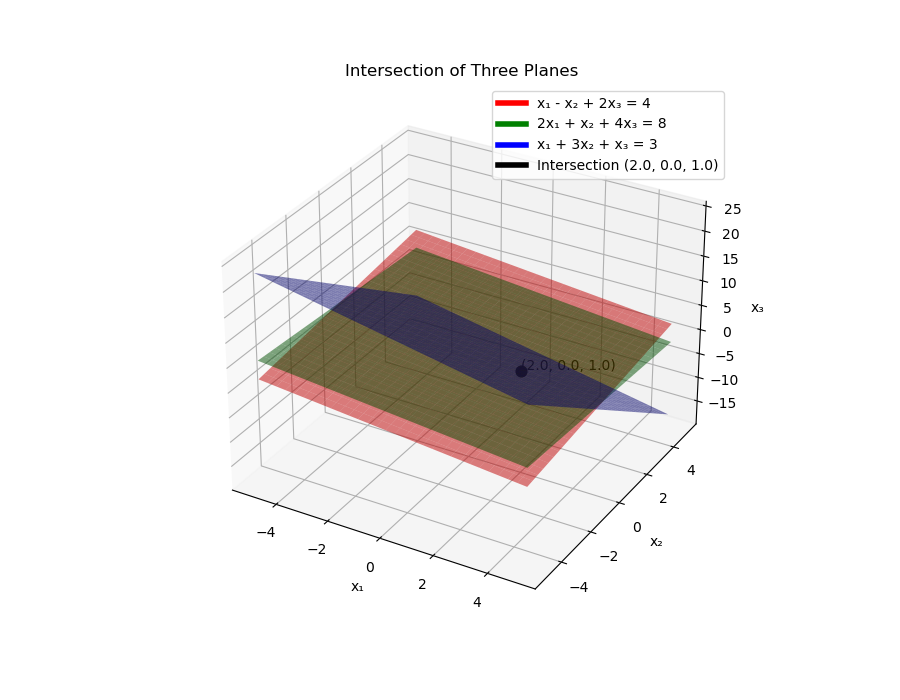
\includegraphics[height=0.5\textheight, keepaspectratio]{figs/Figure_1.png}
    \label{figure_1}
\end{figure}
\end{document}
